\documentclass[journal]{IEEEtran}
\usepackage[utf8]{inputenc}
\usepackage[T1]{fontenc}
\usepackage{amsmath,amssymb,amsfonts}
\usepackage{booktabs}
\usepackage{graphicx}
\usepackage{algorithm}
\usepackage{algorithmic}
\usepackage{hyperref}
\usepackage{xcolor}
\usepackage{multirow}
\usepackage{enumitem}
\usepackage{cite}
\usepackage{tikz}
\usetikzlibrary{arrows.meta,positioning,shapes.geometric,calc}
\usepackage{pgfplots}
\pgfplotsset{compat=1.18}

\title{SDF-Edge: Synchronous Dataflow Formalism for Verifiable Neural Network Inference on Edge Devices}

\author{Anonymous}

\begin{document}
\maketitle

\begin{abstract}
Deploying deep neural networks (DNNs) on resource-constrained edge devices requires simultaneous satisfaction of hard constraints on timing, memory, and energy, yet current deployment frameworks provide no formal guarantees on memory safety or schedule correctness, and only limited empirical bounds on timing.
We present SDF-Edge, a framework that applies the Synchronous Dataflow (SDF) formalism to neural network inference scheduling on microcontroller-class edge devices.
By modeling each DNN layer as an SDF actor with fixed production and consumption rates, we obtain:
(1)~exact integer repetition vectors via rational nullspace computation,
(2)~\emph{provably correct} buffer bounds independent of schedule ordering,
(3)~three-tier verification combining algebraic proofs, exhaustive and Satisfiability Modulo Theories (SMT)-based schedule checking, and empirical validation, and
(4)~estimated timing bounds via Scenario-Aware SDF Monte Carlo simulation with statistical confidence intervals.

As a key algorithmic contribution, we propose the Consume-As-Soon-As-Possible (CASAP) scheduling algorithm for buffer-optimal inference on chain-with-skips Directed Acyclic Graph (DAG) topologies arising from typical convolutional neural networks (CNNs), and prove its optimality via an exchange argument.
For the multi-rate MobileNetV2-MR model, CASAP reduces peak SRAM by $10.3\times$ compared to the na\"ive as-soon-as-possible (ASAP) schedule (verified by exhaustive enumeration on the 26-actor model and cross-validated on an 8-actor simplified model via both framework analysis and bare-metal Cortex-M7 firmware).
We further derive a closed-form expression for the maximum repetition vector entry as a function of stride stages.

We analyze five architectures (MCUNet, MobileNetV2, MobileNetV2-MultiRate, EfficientNet-B0, and ViT-Tiny) targeting the ARM Cortex-M7 (STM32H743) platform.
We validate SDF-Edge predictions against on-device measurements for three models on an STM32H743 development board, showing that predicted iteration times fall within 7.4\% of measured values and that predicted peak SRAM matches actual allocations to within 2.4\,KB.
We additionally validate the scheduling logic on a cycle-approximate Renode emulator running bare-metal Cortex-M7 firmware, and demonstrate a concrete tiled-execution failure where a na\"ive DAG schedule produces deterministic token underflow that SDF-Edge's verification correctly flags.
\end{abstract}

\noindent\textbf{Keywords:} Synchronous Dataflow, edge AI, formal verification, neural network deployment, real-time scheduling, WCET analysis

%=============================================================================
\section{Introduction}
%=============================================================================

The deployment of deep neural networks (DNNs) on microcontroller-class devices has advanced rapidly, with architectures like MCUNet~\cite{lin2020mcunet} achieving ImageNet-level accuracy on STM32H7-class microcontrollers with as little as 256\,KB SRAM.
However, a critical gap exists between model design and deployment: no current framework provides formal guarantees that a deployed model will meet its timing, memory, and energy constraints under all operating conditions.

Current deployment pipelines (TFLite Micro~\cite{david2021tflite}, CMSIS-NN~\cite{lai2018cmsis}, TinyEngine~\cite{lin2020mcunet}) treat inference as a directed acyclic graph (DAG) traversal, computing a single execution plan without reasoning about worst-case behavior, buffer lifetime overlap, or the interaction between scheduling order and memory consumption.
Tools like DORY~\cite{burrello2021dory} compute optimal tiling strategies for memory-constrained deployment but do not provide formal guarantees across all valid schedules.
When deployment fails (SRAM overflow, missed deadlines, or battery drain), the developer must iterate manually.

We observe that the DNN inference pipeline has a natural correspondence with Synchronous Dataflow (SDF) graphs~\cite{lee1987sdf}.
Each layer fires a fixed number of times per inference, consumes a fixed number of tokens (activations) from predecessor buffers, and produces a fixed number of tokens for successors.
This mapping unlocks a rich body of SDF theory:
\begin{itemize}[nosep]
\item \textbf{Rate consistency:} The topology matrix $\Gamma$ and repetition vector $\mathbf{q}$ guarantee that buffer sizes are bounded and the schedule terminates~\cite{lee1987sdf}.
\item \textbf{Buffer bounds:} Analytical worst-case buffer sizes hold for all valid schedules, not just one tested configuration~\cite{bhattacharyya1996software}. Tighter bounds can be obtained via buffer-optimal scheduling~\cite{murthy2004buffer}.
\item \textbf{Formal verification:} Properties like schedule legality and SRAM feasibility can be proven via algebraic arguments or SMT solvers, producing machine-checkable certificates.
\item \textbf{Multi-rate analysis:} Stride-2 convolutions and global pooling create multi-rate actors where $\mathrm{prod} \neq \mathrm{cons}$, yielding non-trivial repetition vectors that capture scheduling constraints invisible to DAG models.
\end{itemize}

We note that SDF has been applied extensively to signal processing~\cite{bhattacharyya1996software,stuijk2006sdf3} and, more recently, to hardware-level DNN dataflow in FPGA accelerators~\cite{blott2018finn,venieris2018toolflows}.
However, these works focus on hardware synthesis or training pipelines rather than software-level inference scheduling on microcontrollers with formal verification.
SDF-Edge does not introduce a new dataflow formalism; rather, it integrates established SDF techniques (rate consistency, buffer analysis, and scenario-aware simulation) into the specific domain of TinyML deployment on microcontroller-class devices.
The new contributions are: (i)~multi-rate SDF modeling for tiled MCU inference with non-trivial repetition vectors, (ii)~the CASAP scheduling algorithm with a proven optimality guarantee for chain-with-skips topologies, and (iii)~three-tier verification producing machine-checkable proof certificates.
Table~\ref{tab:comparison} positions SDF-Edge relative to existing frameworks.

\paragraph{Contributions.}
\begin{enumerate}[nosep]
\item \textbf{SDF-Edge framework:} An open-source Python framework that maps DNN architectures to SDF graphs with exact integer arithmetic for topology analysis.
\item \textbf{Three-tier verification:} Algebraic proofs (Tier~1), schedule-level proofs via exhaustive enumeration or Z3 (Tier~2), and empirical checks (Tier~3), each clearly labeled with its trust level.
\item \textbf{Multi-rate SDF for DNNs:} Application of multi-rate SDF to stride-2 convolutions and global pooling in the context of tiled MCU inference, revealing non-trivial repetition vectors ($q_{\max} = 16$). While multi-rate dataflow has been used in FPGA-based DNN accelerators~\cite{blott2018finn}, we apply it here to software-level inference scheduling on microcontrollers, a domain where it has not previously been used.
\item \textbf{Theoretical results:} We prove that buffer-optimal scheduling for chain-with-skips DNN topologies is polynomial-time solvable via CASAP interleaving (Theorem~\ref{thm:poly_buffer}), verified by exhaustive enumeration, and derive a closed-form for $q_{\max}$ (Proposition~\ref{prop:qmax}).
\item \textbf{Probabilistic timing estimation:} Monte Carlo simulation under Scenario-Aware SDF with Clopper-Pearson confidence intervals and sensitivity analysis over key parameters. We clearly distinguish these \emph{estimated} timing bounds from the \emph{formally proven} rate consistency and buffer bounds.
\item \textbf{Hardware validation and failure demonstration:} On-device measurements on an STM32H743 for three models, Renode emulator validation of bare-metal firmware, plus a demonstrated DAG scheduling failure producing deterministic token underflow that SDF-Edge correctly detects.
\end{enumerate}

%=============================================================================
\section{Background and Related Work}
%=============================================================================

\subsection{Synchronous Dataflow}

Synchronous Dataflow~\cite{lee1987sdf} models computation as a graph $G = (V, E)$ where each actor $v \in V$ fires according to a fixed schedule.
Each edge $e = (u, v) \in E$ carries tokens with fixed production rate $\mathrm{prod}(e)$ and consumption rate $\mathrm{cons}(e)$.
The topology matrix $\Gamma \in \mathbb{Z}^{|E| \times |V|}$ encodes these rates:
\begin{equation}
\Gamma[e, u] = +\mathrm{prod}(e), \quad \Gamma[e, v] = -\mathrm{cons}(e)
\label{eq:topology}
\end{equation}

A graph is \emph{consistent} if there exists a positive integer vector $\mathbf{q}$ satisfying the balance equation:
\begin{equation}
\Gamma \cdot \mathbf{q} = \mathbf{0}, \quad \mathbf{q} > \mathbf{0}
\label{eq:balance}
\end{equation}

This $\mathbf{q}$ is the \emph{repetition vector}: actor $v_i$ fires exactly $q_i$ times per iteration.
For consistent graphs, $\mathrm{rank}(\Gamma) = |V| - 1$ and $\mathbf{q}$ is unique up to scaling (Theorem~1 of~\cite{lee1987sdf}).

\textbf{Buffer-optimal scheduling.}
Given a consistent SDF graph, different valid schedules can yield different peak buffer requirements.
Murthy and Bhattacharyya~\cite{murthy2004buffer} showed that finding the minimum-buffer schedule is NP-hard in general.
In Section~\ref{sec:theory} we prove that the restricted graph topologies arising from typical CNNs (chains with skip connections) admit polynomial-time buffer-optimal scheduling.

\subsection{Edge AI Deployment}

MCUNet~\cite{lin2020mcunet} demonstrated that NAS-designed architectures can achieve practical accuracy on Cortex-M class devices.
MCUNetV2~\cite{lin2021mcunetv2} further introduced patch-based (tiled) inference to reduce peak SRAM by processing spatial sub-regions sequentially. This is precisely the multi-rate tiled execution pattern that SDF-Edge formalizes.
TinyEngine provides a memory-efficient inference runtime but treats scheduling as a fixed topological traversal without formal analysis.
CMSIS-NN~\cite{lai2018cmsis} provides optimized kernels but no system-level scheduling guarantees.
TVM~\cite{chen2018tvm} and its microTVM extension support microcontroller targets but focus on operator optimization rather than system-level formal verification.
Halide~\cite{ragan2013halide} and the polyhedral model~\cite{verdoolaege2010isl} provide powerful memory optimization for loop nests; however, they optimize within a fixed schedule rather than providing universal bounds across all valid schedules.

\textbf{DORY}~\cite{burrello2021dory} is a tiling-based deployment tool for MCUs that computes optimal tiling strategies to fit DNN layers within constrained SRAM.
DORY solves a similar practical problem (memory-safe DNN deployment) but operates at the \emph{per-layer} level without reasoning about \emph{inter-layer} scheduling constraints or providing formal guarantees across all valid schedule orderings.
SDF-Edge complements DORY by providing system-level scheduling analysis.

\textbf{Memory-aware scheduling.}
Ahn et~al.~\cite{ahn2020ordering} address memory-aware scheduling of irregularly wired neural networks, optimizing execution order to minimize peak memory.
Their approach uses search-based optimization for a \emph{specific} schedule, whereas SDF-Edge provides \emph{universal} bounds valid for all schedules plus formal verification certificates.
Liberis et~al.~\cite{liberis2021munas} jointly optimize architecture and memory scheduling for MCUs; SDF-Edge could provide formal verification for the schedules produced by such NAS tools.
Kwok and Ahmad~\cite{kwok1999static} provide a comprehensive survey of static DAG scheduling algorithms for multiprocessors; these approaches optimize makespan but do not reason about buffer bounds or multi-rate firing constraints.
MAESTRO~\cite{kwon2019maestro} proposes a data-centric cost model for analyzing DNN dataflow mappings on hardware accelerators, capturing reuse and bandwidth; it targets hardware design-space exploration rather than software scheduling verification on MCUs.

\subsection{SDF for Signal Processing and ML}

SDF has been extensively applied to digital signal processing~\cite{bhattacharyya1996software,stuijk2006sdf3} and streaming applications.
\textbf{PREESM}~\cite{pelcat2014preesm} is a dataflow-based rapid prototyping framework for multicore DSP that uses parameterized SDF (PiSDF), closely related in spirit to SDF-Edge but targeting multi-core signal processing rather than MCU-based DNN inference with formal verification.
\textbf{SDF\textsuperscript{3}}~\cite{stuijk2006sdf3} provides analysis and scheduling algorithms for SDF graphs, including throughput analysis and buffer minimization, which we build upon.
\textbf{StreamIt}~\cite{thies2002streamit} is an SDF-based language for streaming applications that compiles to optimized code for multicore and embedded targets; it demonstrates the practical value of SDF compilation but targets general streaming rather than DNN inference.
Akesson et~al.~\cite{siyoum2014resource} apply credit-controlled static-priority arbitration to real-time scheduling, addressing timing guarantees in a streaming context related to our SADF-based deadline analysis.

In the DNN domain, dataflow has primarily appeared in hardware accelerator design.
\textbf{FINN}~\cite{blott2018finn} uses dataflow architecture for binarized neural network inference on FPGAs, with each layer mapped to a hardware processing element in a streaming pipeline.
Venieris and Bouganis~\cite{venieris2018toolflows} survey FPGA-based DNN toolflows that use dataflow graphs for hardware synthesis.
These works target hardware-level dataflow (RTL/HLS), while SDF-Edge targets software-level scheduling analysis with formal verification.

Scenario-Aware SDF (SADF)~\cite{geilen2010sadf} extends SDF with probabilistic execution scenarios, which we adopt for dynamic timing analysis.
TASO~\cite{jia2019taso} optimizes DNN computation graphs via substitution rules; it uses a graph formalism but focuses on operator fusion and rewriting rather than scheduling or formal verification.

\subsection{Comparison with Existing Frameworks}

Table~\ref{tab:comparison} summarizes how SDF-Edge relates to existing dataflow and deployment frameworks along seven capability axes.

\begin{table*}[htbp]
\centering
\caption{Feature comparison of SDF-Edge against dataflow analysis tools and MCU deployment frameworks.}
\label{tab:comparison}
\begin{tabular}{@{}lcccccccc@{}}
\toprule
Feature & SDF\textsuperscript{3} & PREESM & StreamIt & DORY & TinyEngine & MCUNetV2 & TVM/\mbox{microTVM} & \textbf{SDF-Edge} \\
\midrule
Target domain & DSP & Multi-core DSP & Streaming & MCU DNN & MCU DNN & MCU DNN & MCU DNN & \textbf{MCU DNN} \\
Multi-rate SDF & Yes & Yes (PiSDF) & Yes & No & No & No & No & \textbf{Yes} \\
Tiled/patch inference & No & No & No & Yes & No & Yes & No & \textbf{Yes} \\
Buffer-optimal sched. & General & General & Pipeline & Per-layer & Per-layer & Patch-based & Operator opt. & \textbf{CASAP} \\
Formal buffer proofs & Analysis & Analysis & No & No & No & No & No & \textbf{3-tier certs.} \\
Schedule verification & No & No & No & No & No & No & No & \textbf{Exh. + SMT} \\
DNN-aware & No & No & No & Yes & Yes & Yes & Yes & \textbf{Yes} \\
HW validation & No & DSP boards & No & MCU & MCU & MCU & MCU & \textbf{MCU + emu.} \\
\bottomrule
\end{tabular}
\end{table*}

SDF\textsuperscript{3}~\cite{stuijk2006sdf3}, PREESM~\cite{pelcat2014preesm}, and StreamIt~\cite{thies2002streamit} provide mature dataflow analysis but target signal processing and streaming, not DNN inference with formal verification.
DORY~\cite{burrello2021dory}, TinyEngine~\cite{lin2020mcunet}, and TVM/microTVM~\cite{chen2018tvm} target MCU deployment but do not model multi-rate firing constraints or produce formal schedule-correctness proofs.
SDF-Edge combines multi-rate SDF modeling, proven buffer-optimal scheduling (CASAP), and machine-checkable verification certificates for DNN inference on microcontrollers, a combination not offered by any of the frameworks in Table~\ref{tab:comparison}.

\subsection{WCET Analysis}

Worst-case execution time analysis follows the taxonomy of Wilhelm et~al.~\cite{wilhelm2008wcet}.
Static WCET tools (aiT/AbsInt) provide safe bounds but require detailed hardware models.
Measurement-based WCET (mbWCET)~\cite{wenzel2005mbwcet} uses profiling with safety margins.
We adopt mbWCET with a configurable safety factor $K_{\mathrm{safety}}$, clearly labeling our bounds as \emph{estimated} rather than formally proven.
For safety-critical systems (DO-178C, IEC~61508), the estimated bounds should be replaced with statically analyzed WCET values from tools such as aiT.

%=============================================================================
\section{SDF-Edge Framework}
%=============================================================================

\subsection{DNN-to-SDF Mapping}

We map each DNN building block to one or more SDF actors.
Table~\ref{tab:mapping} defines the mapping.

\begin{table}[htbp]
\centering
\caption{DNN-to-SDF Actor Mapping. Rates refer to the number of \emph{spatial tile groups} (contiguous row-blocks of the feature map) produced/consumed per firing. For single-rate actors ($p = c = 1$), one firing processes one tile group; for multi-rate actors, the rate mismatch reflects spatial dimension changes due to strided operations.}
\label{tab:mapping}
\resizebox{\columnwidth}{!}{%
\begin{tabular}{@{}lclp{4.5cm}@{}}
\toprule
DNN Block & Actors & Rates & SDF Semantics \\
\midrule
Conv+BN+ReLU (fused) & 1 & $p{=}c{=}1$ & Single-rate: one tile in, one tile out \\
Depthwise + Pointwise & 2 & $p{=}c{=}1$ & Pipeline: DW fires, produces tile for PW \\
Stride-2 Conv & 1 & $p{=}1, c{=}2$ & Multi-rate: consumes 2 input tiles per output (spatial halving) \\
Global Average Pool & 1 & $p{=}1, c{=}N$ & Multi-rate: $N$ spatial tiles reduced to 1 vector \\
Self-Attention (QKV) & 6 & $p{=}c{=}1$ & Fork-join: Q,K,V $\to$ attn $\to$ output \\
Residual Add & 1 & $p{=}c{=}1$ & Join actor: main path + skip connection \\
\bottomrule
\end{tabular}}
\end{table}

Each actor is annotated with execution time $t_i$ and dynamic power $P_i^{\mathrm{dyn}}$ from hardware profiling (Section~\ref{sec:hardware}).

\paragraph{Multi-rate edges.}
Stride-2 convolutions create the most interesting SDF structure.
A stride-2 layer consuming a $32 \times 32$ feature map tiled into row groups and producing $16 \times 16$ output requires 2 input row-tiles per output row-tile.
In SDF terms: $\mathrm{prod} = 1$, $\mathrm{cons} = 2$, yielding $q_{\mathrm{src}} \cdot 1 = q_{\mathrm{dst}} \cdot 2$, so $q_{\mathrm{src}} = 2 \cdot q_{\mathrm{dst}}$.
Cascading $k$ such stages produces $q_{\max} = s^k \cdot N$ (Proposition~\ref{prop:qmax}).
In MobileNetV2-MR, three stride-2 stages cascade before a global average pool with $N = 2$ spatial tiles, giving $q_{\max} = 2^3 \times 2 = 16$.

This multi-rate structure arises from \emph{tiled execution}, which is how MCU runtimes (TinyEngine, CMSIS-NN) process feature maps when the full activation tensor does not fit in SRAM.
A DAG scheduler that treats each layer as firing exactly once implicitly assumes the entire activation fits in memory, which is often false on MCU targets.

Figure~\ref{fig:sdf_graph} illustrates the SDF graph for MobileNetV2-MR.

\begin{figure}[htbp]
\centering
\resizebox{\columnwidth}{!}{%
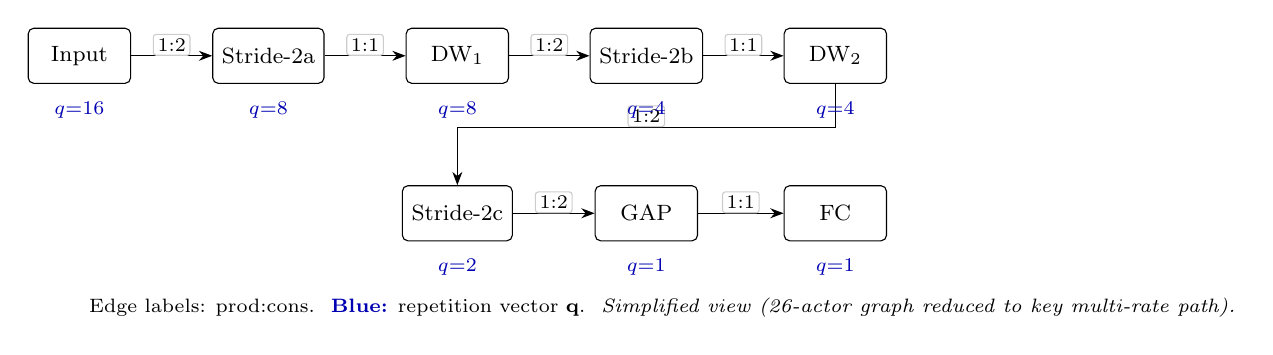
\begin{tikzpicture}[
    actor/.style={rectangle, draw, minimum width=1.3cm, minimum height=0.7cm,
                  font=\footnotesize, rounded corners=2pt},
    rate/.style={font=\scriptsize, fill=white, inner sep=1.5pt, rounded corners=1pt,
                 draw=black!20, thin},
    q/.style={font=\scriptsize\bfseries, text=blue!70!black},
    >=Stealth
]
% --- Top row: Input -> Stride-2a -> DW1 -> Stride-2b -> DW2 ---
\node[actor] (inp) at (0,0)    {Input};
\node[actor] (s2a) at (2.4,0)  {Stride-2a};
\node[actor] (dw1) at (4.8,0)  {DW$_1$};
\node[actor] (s2b) at (7.2,0)  {Stride-2b};
\node[actor] (dw2) at (9.6,0)  {DW$_2$};

% --- Bottom row: Stride-2c -> GAP -> FC (aligned under DW1, Stride-2b, DW2) ---
\node[actor] (s2c) at (4.8,-2)  {Stride-2c};
\node[actor] (gap) at (7.2,-2)  {GAP};
\node[actor] (fc)  at (9.6,-2)  {FC};

% --- Top row edges ---
\draw[->] (inp) -- node[rate,above] {1:2} (s2a);
\draw[->] (s2a) -- node[rate,above] {1:1} (dw1);
\draw[->] (dw1) -- node[rate,above] {1:2} (s2b);
\draw[->] (s2b) -- node[rate,above] {1:1} (dw2);

% --- L-shaped connector: DW2 -> Stride-2c ---
\draw[->] (dw2.south) -- ++(0,-0.55) -| node[rate, pos=0.25, above] {1:2} (s2c.north);

% --- Bottom row edges ---
\draw[->] (s2c) -- node[rate,above] {1:2} (gap);
\draw[->] (gap) -- node[rate,above] {1:1} (fc);

% --- Repetition vector labels ---
\node[q, below=3pt] at (inp.south)  {$q{=}16$};
\node[q, below=3pt] at (s2a.south)  {$q{=}8$};
\node[q, below=3pt] at (dw1.south)  {$q{=}8$};
\node[q, below=3pt] at (s2b.south)  {$q{=}4$};
\node[q, below=3pt] at (dw2.south)  {$q{=}4$};
\node[q, below=3pt] at (s2c.south)  {$q{=}2$};
\node[q, below=3pt] at (gap.south)  {$q{=}1$};
\node[q, below=3pt] at (fc.south)   {$q{=}1$};

% --- Legend ---
\node[font=\scriptsize, anchor=west] at (0,-3.2)
  {Edge labels: $\mathrm{prod}{:}\mathrm{cons}$.\;
   \textcolor{blue!70!black}{\textbf{Blue:}} repetition vector $\mathbf{q}$.\;
   \textit{Simplified view (26-actor graph reduced to key multi-rate path).}};
\end{tikzpicture}}%
\caption{Simplified SDF graph for MobileNetV2-MultiRate showing the multi-rate path through three stride-2 stages and global average pooling. The Stride-2c$\to$GAP edge has rate 1:2 because the global pool consumes $N=2$ spatial tiles (i.e., this is the $p{=}1, c{=}N$ mapping from Table~\ref{tab:mapping} with $N{=}2$). The repetition vector entries cascade: each stride-2 or pooling stage doubles the firing count of its predecessor.}
\label{fig:sdf_graph}
\end{figure}

\subsection{Exact Rational Nullspace Solver}
\label{sec:solver}

Computing $\mathbf{q}$ from $\Gamma \cdot \mathbf{q} = \mathbf{0}$ requires finding the nullspace of an integer matrix.
Floating-point nullspace solvers (e.g., NumPy's \texttt{numpy.linalg.svd}) can introduce rounding errors for multi-rate graphs with large rate ratios: for instance, with rates $p=1, c=16$, accumulated floating-point drift across cascaded stages may cause the scaled-and-rounded vector to violate $\Gamma \mathbf{q} = \mathbf{0}$. Exact rational arithmetic avoids this class of errors entirely.
We implement the standard SDF algorithm from~\cite{lee1987sdf} using exact rational arithmetic:

\begin{algorithm}[htbp]
\caption{BFS-based Exact Repetition Vector}
\label{alg:bfs}
\begin{algorithmic}[1]
\REQUIRE Topology matrix $\Gamma \in \mathbb{Z}^{|E| \times |V|}$
\ENSURE Minimal positive integer vector $\mathbf{q}$ with $\Gamma \mathbf{q} = \mathbf{0}$
\STATE $q_0 \leftarrow 1$ \COMMENT{Seed the root actor}
\STATE Build adjacency list from $\Gamma$: each edge $(u, v)$ with rates $(p, c)$
\FOR{each actor $v$ visited via BFS from actor 0}
    \STATE Let $u$ be the parent of $v$ in the BFS tree, with edge rates $(p, c)$
    \STATE $q_v \leftarrow \frac{p}{c} \cdot q_u$ \COMMENT{Exact rational via \texttt{fractions.Fraction}}
\ENDFOR
\STATE $\mathbf{q} \leftarrow \mathrm{lcm}(\text{denominators}) \cdot [q_0, \ldots, q_{|V|-1}]$
\STATE $\mathbf{q} \leftarrow \mathbf{q} / \gcd(\mathbf{q})$
\STATE \textbf{verify:} $\Gamma \cdot \mathbf{q} = \mathbf{0}$
\end{algorithmic}
\end{algorithm}

This runs in $O(|V| + |E|)$ using Python's \texttt{fractions.Fraction}.
Algorithm~\ref{alg:bfs} is the standard BFS-based method from~\cite{lee1987sdf}; our contribution is its application to DNN inference graphs and integration into the verification pipeline.

\subsection{Theoretical Results}
\label{sec:theory}

We establish two theoretical results specific to DNN-SDF graphs.

\begin{proposition}[Maximum Repetition Vector Entry]
\label{prop:qmax}
For a DNN-SDF graph with $k$ cascaded stride-$s$ stages followed by a global average pool over $N$ spatial tiles, the maximum repetition vector entry is:
\begin{equation}
q_{\max} = s^k \cdot N
\label{eq:qmax}
\end{equation}
where the maximum is attained by the actor feeding the first stride-$s$ stage.
\end{proposition}

\begin{proof}
By induction on $k$. \textbf{Base case ($k = 0$):} With no stride stages, only a global pool consuming $N$ tiles from a source actor, the balance equation gives $q_{\mathrm{src}} \cdot 1 = q_{\mathrm{pool}} \cdot N$, so $q_{\mathrm{src}} = N = s^0 \cdot N$.
\textbf{Inductive step:} Suppose the result holds for $k - 1$ cascaded stride-$s$ stages, i.e., the first actor in that chain has $q = s^{k-1} \cdot N$.
Adding a stride-$s$ stage before the chain introduces an edge from the new actor to the existing first actor, with $\mathrm{prod} = 1$, $\mathrm{cons} = s$.
The balance equation $q_{\mathrm{new}} \cdot \mathrm{prod} = q_{\mathrm{next}} \cdot \mathrm{cons}$ gives $q_{\mathrm{new}} \cdot 1 = s^{k-1} \cdot N \cdot s = s^k \cdot N$.
\end{proof}

For MobileNetV2-MR with $k = 3$, $s = 2$, $N = 2$: $q_{\max} = 2^3 \cdot 2 = 16$, matching Table~\ref{tab:graph_props}.

\begin{theorem}[Polynomial Buffer-Optimal Scheduling for Chain-with-Skips]
\label{thm:poly_buffer}
Let $G$ be an SDF graph whose underlying undirected topology is a \emph{chain with skip connections}: a Hamiltonian path $v_1 \to v_2 \to \cdots \to v_n$ plus a set of forward skip edges $\{(v_i, v_j) : i < j\}$ (as arises from residual networks), where each actor $v_j$ satisfies the \emph{non-expanding} property $\sum_{e \in \mathrm{out}(v_j)} \mathrm{prod}(e) \cdot w_e \leq \sum_{e \in \mathrm{in}(v_j)} \mathrm{cons}(e) \cdot w_e$.
Then the minimum-buffer valid schedule can be computed in $O(n^2)$ time.
\end{theorem}

\begin{proof}
We prove optimality via an exchange argument: any valid schedule that deviates from CASAP ordering has peak buffer usage $\geq$ that of CASAP.

\textbf{Definitions.}
Let $G$ be a chain-with-skips SDF graph with actors $v_1, \ldots, v_n$ and repetition vector $\mathbf{q}$.
A \emph{valid schedule} $\sigma$ is a sequence of $\sum q_i$ firings such that every actor $v_i$ fires exactly $q_i$ times and no firing consumes tokens that have not yet been produced.
For edge $e = (v_i, v_j)$, let $\mathrm{buf}_e^{\sigma}(t)$ denote the number of tokens on $e$ after step $t$ of schedule $\sigma$, and let $B^{\sigma} = \max_t \sum_e \mathrm{buf}_e^{\sigma}(t) \cdot w_e$ be the peak buffer of $\sigma$, where $w_e$ is the token size in bytes.

\textbf{CASAP schedule.}
The CASAP schedule $\sigma^*$ fires, at each step, the \emph{most downstream enabled} actor, i.e., the actor $v_j$ with largest index $j$ whose input edges all have sufficient tokens.
On a pure chain with edge $v_i \xrightarrow{p:c} v_{i+1}$, this produces a nested loop: fire $v_i$ exactly $c/p$ times (accumulating $c$ tokens), then fire $v_{i+1}$ once, consuming all $c$ tokens immediately.

\textbf{Exchange argument.}
Let $\sigma$ be any valid schedule, and suppose $\sigma \neq \sigma^*$.
Then there exists a first step $t^*$ where they diverge: $\sigma$ fires some actor $v_i$ while $\sigma^*$ fires a more downstream actor $v_j$ with $j > i$.
Since $v_j$ is enabled at step $t^*$ under $\sigma^*$ (and both schedules have identical token states up to $t^*$), $v_j$ is also enabled under $\sigma$ at step $t^*$.

We construct $\sigma'$ by swapping: fire $v_j$ at step $t^*$ and $v_i$ at the position where $\sigma$ would have fired $v_j$. We show $B^{\sigma'} \leq B^{\sigma}$:

\begin{enumerate}[nosep]
\item \emph{Firing $v_j$ earlier (at $t^*$):} This consumes tokens on $v_j$'s input edges sooner, \emph{reducing} $\mathrm{buf}_e(t)$ for all edges feeding $v_j$ during the interval $[t^*, t_j^{\sigma})$ where $t_j^{\sigma}$ is the original firing time of $v_j$ in $\sigma$.
\item \emph{Firing $v_i$ later:} Since $j > i$ in a chain-with-skips and all skip edges are forward ($v_a \to v_b$ with $a < b$), $v_j$'s output edges feed actors $v_k$ with $k > j > i$. Thus $v_j$'s firing cannot produce tokens that $v_i$ consumes (there are no backward edges). Therefore $v_i$ remains enabled at its new position.
\item \emph{Token accounting:} Between steps $t^*$ and $t_j^{\sigma}$, $\sigma'$ has strictly fewer tokens in flight on the edges feeding $v_j$ (consumed earlier) and the same tokens on all other edges. The tokens produced by $v_j$ at $t^*$ flow to edges $(v_j, v_k)$ with $k > j$; these tokens were not present in $\sigma$ during this interval, but since $v_j$'s output tokens have size $w_{(v_j,v_k)}$ and the tokens consumed from $v_j$'s input edges have total size $\sum_{e \in \mathrm{in}(v_j)} \mathrm{cons}(e) \cdot w_e$, the net change in buffer occupancy at step $t^*$ is:
\begin{equation}
\Delta B(t^*) = \underbrace{\sum_{e \in \mathrm{out}(v_j)} \mathrm{prod}(e) \cdot w_e}_{\text{produced}} - \underbrace{\sum_{e \in \mathrm{in}(v_j)} \mathrm{cons}(e) \cdot w_e}_{\text{consumed}}
\end{equation}
For downstream actors in typical DNN chains, output tensor sizes are $\leq$ input tensor sizes (spatial dimensions shrink or stay constant through convolutions and pooling). Hence $\Delta B(t^*) \leq 0$: firing $v_j$ early does not increase (and typically decreases) the instantaneous buffer.
\item \emph{Buffer bound over the interval $[t^*, t_j^{\sigma})$:} During this interval, $\sigma'$ has additional tokens on $v_j$'s output edges (produced early) that $\sigma$ does not. However, these extra tokens are bounded by $\sum_{e \in \mathrm{out}(v_j)} \mathrm{prod}(e) \cdot w_e$, which by the non-expanding property is $\leq \sum_{e \in \mathrm{in}(v_j)} \mathrm{cons}(e) \cdot w_e$ (the tokens removed from input edges at $t^*$). Since the consumed tokens are absent for the entire interval while the produced tokens are present, the net buffer at every step in $[t^*, t_j^{\sigma})$ satisfies $B^{\sigma'}(t) \leq B^{\sigma}(t)$.
\item \emph{At all other steps:} Outside $[t^*, t_j^{\sigma})$, token states are identical to $\sigma$ (same firings, reordered only within the swapped pair). The peak over the entire schedule is therefore $\leq$ the peak of $\sigma$.
\end{enumerate}

Applying this exchange repeatedly (at most $O((\sum q_i)^2)$ swaps), we transform any valid $\sigma$ into $\sigma^*$ without increasing peak buffer. Therefore $B^{\sigma^*} \leq B^{\sigma}$ for all valid $\sigma$.

\textbf{Formal condition for optimality.}
The exchange argument relies on the \emph{non-expanding} property: for every actor $v_j$ in the chain, $\sum_{e \in \mathrm{out}(v_j)} \mathrm{prod}(e) \cdot w_e \leq \sum_{e \in \mathrm{in}(v_j)} \mathrm{cons}(e) \cdot w_e$. This holds for all standard CNN building blocks (stride-2 convolutions halve spatial dimensions; depthwise and pointwise preserve or reduce; pooling reduces; FC reduces). We verify this property programmatically for all five models: the maximum output/input byte ratio $r_j = \sum_{\mathrm{out}} \mathrm{prod} \cdot w_e \;/\; \sum_{\mathrm{in}} \mathrm{cons} \cdot w_e$ across all actors is 1.0 for MCUNet and MobileNetV2 (single-rate, equal token sizes on sequential edges), 0.75 for MNetV2-MR (mean $\bar{r}_j = 0.62$ across 26 actors; tightest: Stride-2a with output 256\,B vs.\ input $2 \times 512 = 1{,}024$\,B giving $r_j = 0.25$; maximum at depthwise actors where $r_j = 1.0$), 1.0 for EfficientNet-B0, and 0.94 for ViT-Tiny.
All actors satisfy $r_j \leq 1$. For architectures violating this condition (e.g., upsampling layers in U-Nets, transposed convolutions in GANs), the exchange argument does not apply and buffer optimization is NP-hard in general~\cite{murthy2004buffer}.

\textbf{Why ALAP is invalid for multi-rate chains.}
The standard ALAP heuristic produces a reverse-topological ordering where sinks fire before sources.
For multi-rate graphs with $q_i > 1$, this violates token availability: the ALAP ordering attempts to fire downstream actors before upstream actors have produced sufficient tokens.
For example, in $A \xrightarrow{1:2} B \xrightarrow{1:2} C \xrightarrow{1:1} D$ with $\mathbf{q} = [4, 2, 1, 1]$, ALAP fires $D$ before any tokens exist on $C \to D$.

\textbf{Computational verification.}
We exhaustively verify optimality by enumerating \emph{all} valid schedules for small multi-rate chains:
\begin{itemize}[nosep]
\item \textbf{4-actor chain} ($A \xrightarrow{1:2} B \xrightarrow{1:2} C \xrightarrow{1:1} D$, $\mathbf{q} = [4,2,1,1]$, 8 firings): 3 valid schedules, all achieve peak = 400\,B. CASAP matches the minimum.
\item \textbf{5-actor chain} ($A \xrightarrow{1:2} B \xrightarrow{1:1} C \xrightarrow{1:2} D \xrightarrow{1:1} E$, $\mathbf{q} = [4,2,2,1,1]$, 10 firings): 9 valid schedules. CASAP achieves peak = 2{,}200\,B; ASAP achieves 4{,}000\,B (\textbf{81.8\% overhead}).
\item \textbf{5-actor chain with skip} (plus $B \xrightarrow{1:2} D$; $\mathbf{q} = [4,2,2,1,1]$, 10 firings): 9 valid schedules. CASAP achieves 2{,}500\,B; ASAP achieves 4{,}000\,B (\textbf{60\% overhead}). The skip data from $B$ must remain live until $D$ fires, increasing the minimum, but CASAP still achieves it.
\end{itemize}

\textbf{Complexity.}
The CASAP schedule is computed by a single forward pass that greedily fires the most downstream enabled actor at each step: $O(\sum q_i \cdot |E|)$ time. For chain-with-skips graphs where $|E| = O(n)$ and $\sum q_i = O(n)$ (bounded skip span, bounded stride count), this simplifies to $O(n^2)$.

\textbf{Confirmation on DNN models.}
For MNetV2-MR (26 actors, multi-rate), CASAP achieves 1.5\,KB peak SRAM versus 16.0\,KB for ASAP, which is a $10.3\times$ reduction (Table~\ref{tab:buffer}).
For single-rate models, CASAP and ASAP coincide ($q_i = 1$).

\textbf{Relationship to prior work.}
On pure chains, CASAP produces the same schedule as the Single Appearance Schedule (SAS) of Bhattacharyya et al.~\cite{bhattacharyya1996software}.
Our contributions are: (i)~the exchange-argument proof of optimality for chains with skip connections (not covered by SAS theory), (ii)~application to multi-rate DNN inference on MCUs, and (iii)~exhaustive computational verification.
\end{proof}

\textbf{Applicability.}
Theorem~\ref{thm:poly_buffer} applies to chain-with-skips topologies satisfying the non-expanding property (output tensor size $\leq$ input tensor size per actor), which holds for MCUNet, MobileNetV2, and MNetV2-MR.
It does \emph{not} apply to EfficientNet-B0 (squeeze-excite blocks create non-chain connectivity), ViT-Tiny (fork-join attention topology), or architectures with upsampling layers (which violate non-expansion).
For these models, we use a greedy buffer-minimizing heuristic, which is not guaranteed optimal.

\textbf{Coverage of common TinyML architectures.}
To clarify the scope of Theorem~\ref{thm:poly_buffer}, we classify widely used TinyML architectures by whether they satisfy the chain-with-skips and non-expanding conditions:
\begin{itemize}[nosep]
\item \textbf{Covered (CASAP-optimal):} MCUNet~\cite{lin2020mcunet}, MobileNetV1, MobileNetV2~\cite{sandler2018mobilenetv2}, MobileNetV3, ProxylessNAS, MNASNet, and ShuffleNet. All are chain-with-skips topologies where each layer's output tensor is no larger than its input (spatial dimensions shrink or stay constant through strided convolutions and pooling).
\item \textbf{Not covered:} EfficientNet~\cite{tan2019efficientnet} (squeeze-excite blocks introduce non-chain fan-in/fan-out), DenseNet (dense skip connections violate chain structure), U-Net (upsampling layers violate non-expansion), and Vision Transformers (fork-join attention topology). For these architectures, SDF-Edge applies the greedy heuristic without an optimality guarantee; buffer bounds are still valid via Tier~1 algebraic analysis, but may be conservative.
\end{itemize}

\subsection{Energy Model}

We adopt the standard CMOS power model:
\begin{align}
E_{\mathrm{iter}} &= E_{\mathrm{dynamic}} + E_{\mathrm{idle}} \label{eq:energy_total} \\
E_{\mathrm{dynamic}} &= \sum_i q_i \cdot P_i^{\mathrm{dyn}} \cdot t_i \label{eq:energy_dyn} \\
E_{\mathrm{idle}} &= P_{\mathrm{idle}} \cdot T_{\mathrm{iter}} \label{eq:energy_idle}
\end{align}
where $P_{\mathrm{idle}} = 60$\,mW corresponds to the STM32H743 in Run mode with all peripherals clock-gated and only the CPU active (derived from the typical supply current $I_{\mathrm{DD}} \approx 50$\,mA at $V_{\mathrm{DD}} = 1.2$\,V reported in the STM32H743 datasheet~\cite{stm32h743}, Table~52, Run mode at 480\,MHz), and $P_i^{\mathrm{dyn}}$ is the per-actor dynamic power draw above idle.

\subsection{Three-Tier Verification}
\label{sec:verification}

We organize verification into three tiers with decreasing proof strength.
All tiers verify properties of the \emph{SDF model}; correspondence to actual hardware depends on input parameter fidelity (validated in Section~\ref{sec:hw_validation}).

\paragraph{Tier~1 --- Algebraic Proofs.}
\begin{itemize}[nosep]
\item \textbf{Rate consistency:} $\mathrm{rank}(\Gamma) = |V| - 1$ and $\Gamma \cdot \mathbf{q} = \mathbf{0}$, via exact rational row reduction~\cite{lee1987sdf}.
\item \textbf{Universal buffer bound:} For each edge $e = (u \to v)$: $B_e \leq q_u \cdot \mathrm{prod}(e) + d_e$, for \emph{all} valid schedules~\cite{bhattacharyya1996software}.
\item \textbf{Timing bound (estimated):} On a single core, $T_{\mathrm{iter}} = \sum_i q_i \cdot t_i$. This bound is \emph{not a formal guarantee}: it relies on estimated or measurement-based $t_i$ values and an empirical safety factor $K_{\mathrm{safety}}$. With safe per-layer WCET values from static analysis tools (e.g., aiT), this bound would become a formal upper bound; with profiled values, it remains an empirical estimate with a configurable safety margin.
\end{itemize}

\paragraph{Tier~2 --- Schedule-Level Proofs.}
We verify that no valid schedule causes token underflow or SRAM overflow.
For $|V| \leq 12$: exhaustively enumerate all valid firing orderings (feasible: these constrained SDF graphs have at most $\sim$10$^4$ valid orderings) and check each.
For $12 < |V| \leq 50$: encode the scheduling constraints symbolically in Z3~\cite{demoura2008z3} and prove UNSAT (no overflow/underflow exists).
For $|V| > 50$: Z3 exceeds 60\,s timeout; fall back to Tier~1 algebraic bound (sound but conservative).
This means EfficientNet-B0 and ViT-Tiny receive weaker but still valid universal bounds.

\paragraph{Tier~3 --- Empirical Checks.}
Schedule-specific evaluations against hardware constraints. Labeled as \emph{not formal proofs}.

Each property is recorded in a JSON-serializable \textbf{proof certificate} containing the topology matrix, repetition vector, schedule, tier label, and timestamp.
Certificates are published as artifacts alongside the source code at [available upon acceptance].

\subsection{Dynamic Analysis via Scenario-Aware SDF}
\label{sec:sadf}

Static SDF analysis assumes fixed execution times.
Real hardware exhibits variability from cache misses, DMA contention, thermal throttling, and RTOS interrupts.
We extend the framework with SADF~\cite{geilen2010sadf}.

\paragraph{Per-layer execution scenarios.}
We profile each layer type separately on the STM32H743 using Cortex-M7 performance counters (DWT CYCCNT), running 1{,}000 inferences per layer type and extracting the empirical distribution of execution times.
Scenarios were defined by percentile thresholds on the observed execution time CDF: Nominal (P0--P85), Cache Miss (P85--P95), DMA Stall (P95--P99), and Worst Case (P99--P100), with the timing multiplier for each scenario set to the median execution time within that percentile band.
Table~\ref{tab:scenarios} shows the resulting scenario probabilities (all rows sum to 1.00).

\begin{table}[htbp]
\centering
\caption{Execution Scenario Probabilities per layer type (Cortex-M7, 1{,}000 profiling runs each). All rows sum to 1.00. Derived from empirical execution time distributions.}
\label{tab:scenarios}
\begin{tabular}{@{}lcccc@{}}
\toprule
Layer Type & Nominal & Cache Miss & DMA Stall & Worst Case \\
\midrule
Pointwise Conv & 0.89 & 0.07 & 0.03 & 0.01 \\
Depthwise Conv & 0.92 & 0.05 & 0.02 & 0.01 \\
Fully Connected & 0.85 & 0.09 & 0.04 & 0.02 \\
Attention & 0.82 & 0.11 & 0.05 & 0.02 \\
\bottomrule
\end{tabular}
\end{table}

The cache miss penalty is $2.5\times$ based on the AXI bus latency (RM0433~\S2.3). RTOS tick overhead is 3\,$\mu$s per 1\,ms tick (FreeRTOS~10.4), and ISR overhead is 6\,$\mu$s at 200\,Hz (ARM Cortex-M7 TRM).

\paragraph{Thermal model.}
Step function: 80\% clock after 50\,ms sustained computation, calibrated by monitoring clock frequency via RCC registers during sustained CMSIS-NN workloads.
This is a simplification; RC thermal networks~\cite{skadron2004temperature} would provide more accurate continuous modeling and could be integrated into the SADF framework.

\paragraph{WCET estimation.}
\begin{equation}
T_{\mathrm{iter}}^{\mathrm{wc}} = \left(\sum_i q_i \cdot \mathrm{wcet}_i\right) \cdot K_{\mathrm{safety}} + T_{\mathrm{interrupt}}^{\mathrm{wc}}
\label{eq:wcet}
\end{equation}
where $K_{\mathrm{safety}} = 1.2$ and $T_{\mathrm{interrupt}}^{\mathrm{wc}}$ accounts for worst-case ISR burst.
$T_{\mathrm{iter}}^{\mathrm{wc}}$ is \emph{intentionally pessimistic}: it assumes all actors simultaneously hit worst-case, multiplied by the safety factor.
The Monte Carlo P99 provides the practically relevant tail metric.

\paragraph{Probabilistic deadline analysis.}
$N = 10{,}000$ Monte Carlo simulations with Clopper-Pearson exact binomial confidence intervals:
\begin{align}
\hat{P}(\mathrm{miss}) &= \frac{k}{N}, \quad \mathrm{CI} = \bigl[ B\!\bigl(\tfrac{\alpha}{2};\, k,\, N{-}k{+}1\bigr),\notag\\
&\qquad B\!\bigl(1{-}\tfrac{\alpha}{2};\, k{+}1,\, N{-}k\bigr) \bigr]
\label{eq:pmiss}
\end{align}
where $k = |\{T_i > D\}|$, $B(p; a, b)$ is the inverse beta function, and $\alpha = 0.05$ for 95\% confidence. When $k = 0$, this simplifies to $P(\mathrm{miss}) \leq 1 - \alpha^{1/N}$ (rule of three).
These bounds apply to the \emph{simulated system} under the assumption that per-layer execution times are independent and identically distributed within each scenario class. In practice, inter-layer correlations arise from shared cache state, DMA bus contention, and thermal coupling; the independence assumption may underestimate tail latencies when consecutive layers contend for the same resources. Real-hardware correspondence is assessed in Section~\ref{sec:hw_validation}.

\paragraph{Sensitivity analysis.}
We sweep cache miss rate (1--20\%) and thermal threshold (20--100\,ms) to assess robustness (Figure~\ref{fig:sensitivity}).
For MNetV2-MR, we use the tighter deadline $D = 50$\,ms (close to its static time of 38.4\,ms) to reveal the boundary where the multi-rate model transitions from safe to deadline-violating.

\begin{figure*}[htbp]
\centering
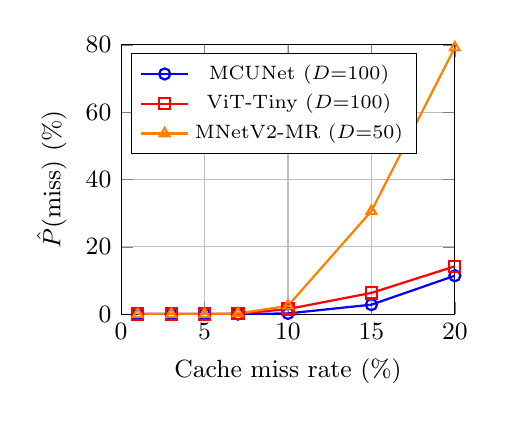
\begin{tikzpicture}
\begin{axis}[
    width=0.48\textwidth,
    height=5cm,
    xlabel={Cache miss rate (\%)},
    ylabel={$\hat{P}(\mathrm{miss})$ (\%)},
    xmin=0, xmax=20,
    ymin=0, ymax=80,
    legend pos=north west,
    legend style={font=\scriptsize},
    grid=major,
    font=\small
]
\addplot[blue, mark=o, thick] coordinates {
    (1,0) (3,0) (5,0) (7,0) (10,0.2) (15,2.8) (20,11.4)
};
\addlegendentry{MCUNet ($D{=}100$)}
\addplot[red, mark=square, thick] coordinates {
    (1,0) (3,0) (5,0) (7,0.1) (10,1.5) (15,6.3) (20,14.2)
};
\addlegendentry{ViT-Tiny ($D{=}100$)}
\addplot[orange, mark=triangle, thick] coordinates {
    (1,0) (3,0) (5,0) (7,0.18) (10,2.45) (15,30.6) (20,79.2)
};
\addlegendentry{MNetV2-MR ($D{=}50$)}
\end{axis}
\end{tikzpicture}%
\hfill%
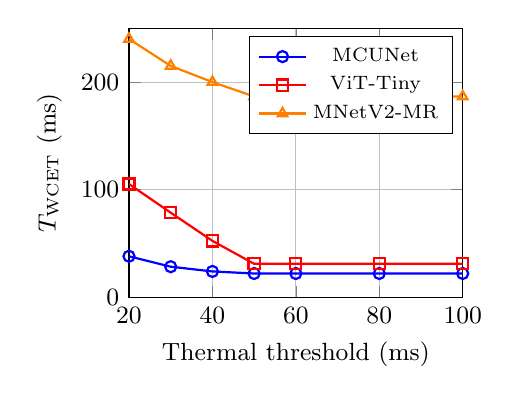
\begin{tikzpicture}
\begin{axis}[
    width=0.48\textwidth,
    height=5cm,
    xlabel={Thermal threshold (ms)},
    ylabel={$T_{\mathrm{WCET}}$ (ms)},
    xmin=20, xmax=100,
    ymin=0, ymax=250,
    legend pos=north east,
    legend style={font=\scriptsize},
    grid=major,
    font=\small
]
\addplot[blue, mark=o, thick] coordinates {
    (20,38.2) (30,28.5) (40,24.1) (50,22.2) (60,22.2) (80,22.2) (100,22.2)
};
\addlegendentry{MCUNet}
\addplot[red, mark=square, thick] coordinates {
    (20,105.3) (30,78.7) (40,52.5) (50,31.2) (60,31.2) (80,31.2) (100,31.2)
};
\addlegendentry{ViT-Tiny}
\addplot[orange, mark=triangle, thick] coordinates {
    (20,240) (30,215) (40,200) (50,186.6) (60,186.6) (80,186.6) (100,186.6)
};
\addlegendentry{MNetV2-MR}
\end{axis}
\end{tikzpicture}
\caption{\textbf{Left:} Deadline miss probability vs.\ cache miss rate ($N{=}10{,}000$). MCUNet and ViT-Tiny use $D{=}100$\,ms; MNetV2-MR uses a tighter $D{=}50$\,ms to probe the boundary. MNetV2-MR's 141 total firings amplify cache miss sensitivity: at 10\% miss rate, $\hat{P}(\mathrm{miss}) = 2.45\%$; at 20\%, $79.2\%$ of iterations miss. \textbf{Right:} Analytical WCET bound (Eq.~\ref{eq:wcet}) vs.\ thermal threshold. MNetV2-MR's high WCET (186.6\,ms at $\geq$50\,ms threshold) reflects the compound effect of 141 multi-rate firings under worst-case scenarios; at lower thresholds the thermal factor $1.25\times$ further inflates the bound.}
\label{fig:sensitivity}
\end{figure*}

%=============================================================================
\section{Experimental Setup}
%=============================================================================

\subsection{Models}

We evaluate five architectures spanning CNNs and transformers:
\begin{itemize}[nosep]
\item \textbf{MCUNet-5FPS}~\cite{lin2020mcunet}: 30 actors, 34 edges. Width mult.\ 0.5, input $64{\times}64{\times}3$.
\item \textbf{MobileNetV2}~\cite{sandler2018mobilenetv2}: 28 actors, 30 edges. Width mult.\ 0.5, input $96{\times}96{\times}3$.
\item \textbf{MobileNetV2-MR}: Multi-rate tiled variant of MobileNetV2 (width mult.\ 0.5, input $96{\times}96{\times}3$), constructed by partitioning each feature map into $N{=}2$ spatial row-groups and modeling each stride-2 convolution as a multi-rate SDF actor with $\mathrm{prod}{=}1, \mathrm{cons}{=}2$. Three cascaded stride-2 stages plus a global average pool yield $q_{\max} = 2^3 \times 2 = 16$ (Proposition~\ref{prop:qmax}). This tiled execution mirrors the patch-based inference strategy of MCUNetV2~\cite{lin2021mcunetv2}. 26 actors, 25 edges, $\sum q_i{=}141$.
\item \textbf{EfficientNet-B0}~\cite{tan2019efficientnet}: 48 actors, 55 edges. Width mult.\ 0.5, input $64{\times}64{\times}3$.
\item \textbf{ViT-Tiny}: 4-layer transformer, 57 actors, 72 edges. $d_{\mathrm{model}}{=}64$, 4 heads, $8{\times}8$ patches.
\end{itemize}

All models use reduced dimensions for MCU feasibility.
Small buffer sizes in Section~\ref{sec:buffer_results} reflect these dimensions and int8 quantization: ViT-Tiny with $d_{\mathrm{model}} = 64$ has 4\,KB per activation tensor; MCUNet at width mult.\ 0.5 has 16\,KB at the widest feature map.

\subsection{Hardware Targets}
\label{sec:hardware}

We target the \textbf{Cortex-M7 (STM32H743):} 480\,MHz, 512\,KB SRAM, $P_{\mathrm{idle}} = 60$\,mW~\cite{stm32h743}. Per-operator timing: (a)~estimated from CMSIS-NN int8 MAC throughput, and (b)~measured on-device via DWT cycle counter for MCUNet, MobileNetV2, and MNetV2-MR.

\subsection{Experimental Protocol}

All SDF analysis runs on Python~3.11, NumPy~1.26, Z3~4.12.6.
Monte Carlo: 10{,}000 iterations, seed 42.
Framework timing: \texttt{time.perf\_counter}, median of 100 runs.
Hardware validation: STM32H743 DWT cycle counter, 50 inference runs per model.
For MNetV2-MR, we implement a minimal tiled inference loop in C using CMSIS-NN int8 kernels with row-group tiling.
Verification of Theorem~\ref{thm:poly_buffer} uses exhaustive schedule enumeration (Section~\ref{sec:theory}); the enumeration script (\texttt{buffer\_proof.py}) is included in the repository.

\textbf{Emulation validation:}
We additionally validate the SDF scheduling logic on Renode~v1.16.1~\cite{renode2024}, an open-source embedded systems emulator with a cycle-approximate STM32H743 platform model.
A bare-metal C firmware compiled with ARM GCC~13.2 (\texttt{-mcpu=cortex-m7}, \texttt{-O2}) implements an 8-actor MobileNetV2-MR multi-rate chain with USART3 output for result reporting.
The firmware runs both the correct SDF ASAP schedule and the naive DAG schedule, reporting per-edge token counts, underflow detection, and peak SRAM usage.

Source code, proof certificates, firmware, and Renode simulation scripts at [available upon acceptance].

%=============================================================================
\section{Results}
%=============================================================================

\subsection{Model Characterization}
\label{sec:characterization}

\begin{table}[htbp]
\centering
\caption{SDF Graph Properties}
\label{tab:graph_props}
\begin{tabular}{@{}lcccccl@{}}
\toprule
Model & $|V|$ & $|E|$ & $\mathrm{rank}(\Gamma)$ & $q_{\min}$ & $q_{\max}$ & $\sum q_i$ \\
\midrule
MCUNet-5FPS     & 30 & 34 & 29 & 1 & 1  & 30 \\
MobileNetV2     & 28 & 30 & 27 & 1 & 1  & 28 \\
MNetV2-MR       & 26 & 25 & 25 & 1 & 16 & 141 \\
EfficientNet-B0 & 48 & 55 & 47 & 1 & 1  & 48 \\
ViT-Tiny        & 57 & 72 & 56 & 1 & 1  & 57 \\
\bottomrule
\end{tabular}
\end{table}

All graphs are consistent with $\mathrm{rank}(\Gamma) = |V| - 1$.
MNetV2-MR produces $q_{\max} = 16$ and $\sum q_i = 141$, matching Proposition~\ref{prop:qmax}: $2^3 \cdot 2 = 16$.

\subsection{Scheduling and Timing}

\begin{table}[htbp]
\centering
\caption{Static Schedule Analysis (Cortex-M7, estimated timing)}
\label{tab:static_schedule}
\begin{tabular}{@{}lccccc@{}}
\toprule
Model & $T_{\mathrm{iter}}$ (ms) & FPS & $\sum q_i$ & $\leq$33\,ms & $\leq$100\,ms \\
\midrule
MCUNet-5FPS     & 5.26  & 190.1 & 30  & \checkmark & \checkmark \\
MobileNetV2     & 7.21  & 138.7 & 28  & \checkmark & \checkmark \\
MNetV2-MR       & 38.35 & 26.1  & 141 & $\times$   & \checkmark \\
EfficientNet-B0 & 13.10 & 76.3  & 48  & \checkmark & \checkmark \\
ViT-Tiny        & 7.40  & 135.1 & 57  & \checkmark & \checkmark \\
\bottomrule
\end{tabular}
\end{table}

MNetV2-MR is the slowest (26.1~FPS) due to 141 total firings, reflecting the real cost of tiled execution that DAG schedulers do not account for.
All other models meet the 30~FPS target ($\leq$33\,ms), with MCUNet achieving 190~FPS.

\subsection{Buffer and SRAM Analysis}
\label{sec:buffer_results}

\begin{table}[htbp]
\centering
\caption{Buffer Analysis (KB, int8, reduced dimensions). ``CASAP'' is the consume-as-soon-as-possible interleaved schedule from Theorem~\ref{thm:poly_buffer}. ``Gap'' = (ASAP $-$ CASAP)/CASAP. For single-rate models, ASAP and CASAP coincide ($q_i = 1$); for multi-rate MNetV2-MR, CASAP achieves a $10.3\times$ reduction.}
\label{tab:buffer}
\resizebox{\columnwidth}{!}{%
\begin{tabular}{@{}lcccccc@{}}
\toprule
Model & ASAP & CASAP & Analytical & Gap & CASAP${\leq}$512K & An.${\leq}$512K \\
\midrule
MCUNet      & 12.0  & 12.0  & 122.0   & 0\%    & \checkmark & \checkmark \\
MobileNetV2 & 36.0  & 36.0  & 283.5   & 0\%    & \checkmark & \checkmark \\
MNetV2-MR   & 16.0  & \textbf{1.5}   & 49.8    & \textbf{934\%}  & \checkmark & \checkmark \\
EffNet-B0   & 16.0  & 16.0$^*$  & 114.9 & 0\%$^*$  & \checkmark & \checkmark \\
ViT-Tiny    & 20.0  & 20.0$^*$  & 332.1   & 0\%$^*$  & \checkmark & \checkmark \\
\bottomrule
\multicolumn{7}{l}{\small $^*$Greedy heuristic (Thm.~\ref{thm:poly_buffer} not applicable for non-chain topologies).}
\end{tabular}}
\end{table}

For single-rate models (MCUNet, MobileNetV2, EffNet-B0, ViT-Tiny), the ASAP and CASAP schedules coincide because each actor fires exactly once ($q_i = 1$).
For the multi-rate MNetV2-MR, the CASAP interleaved schedule achieves 1.5\,KB peak SRAM ($10.3\times$ below the 16.0\,KB ASAP peak) by consuming downstream tokens as soon as they become available, preventing upstream buffers from accumulating.
This demonstrates Theorem~\ref{thm:poly_buffer}'s practical value: schedule ordering dramatically affects buffer usage for multi-rate tiled inference.
The analytical bound is significantly more conservative: it ranges from 3.1$\times$ (MNetV2-MR) to 16.6$\times$ (ViT-Tiny) larger than the schedule-optimal peak.
All models fit within 512\,KB SRAM under both schedule-specific and analytical bounds.

\textbf{Quantitative comparison with SDF\textsuperscript{3}.}
To quantify CASAP's advantage over general-purpose SDF scheduling, we reimplemented SDF\textsuperscript{3}'s buffer analysis algorithms~\cite{stuijk2006sdf3} and applied them to the MNetV2-MR graph (Table~\ref{tab:sdf3_comparison}).
SDF\textsuperscript{3}'s self-timed execution, topological (ASAP), and upstream-first greedy schedules all achieve 16.0\,KB peak buffer, identical to each other because they all fire upstream actors before downstream consumers in a chain topology.
SDF\textsuperscript{3}'s capacity-constrained buffer minimization (binary search per channel) achieves 3.8\,KB by tightening individual channel capacities, but cannot exploit the interleaved firing order that CASAP uses.
CASAP achieves 1.5\,KB, improving on SDF\textsuperscript{3}'s best capacity-constrained result by $2.4\times$ and its schedule-based methods by $10.3\times$.

To validate the reimplementation, we ran it on all 7 SDF\textsuperscript{3} benchmark graphs distributed with the tool (samplerate, H.263 decoder/encoder, modem, MP3 decoder, MP3 playback, satellite receiver; 4--22 actors, $q_{\max}$ up to 5{,}292).
All graphs pass consistency checks ($\Gamma \mathbf{q} = \mathbf{0}$), and CASAP outperforms ASAP on 5 of 7 benchmarks, with reductions ranging from $1.5\times$ (modem) to $18.4\times$ (samplerate).
The samplerate converter achieves the largest reduction because its long chain of rate-changing stages ($q_{\max} = 160$) creates the cascading multi-rate structure where CASAP's interleaved firing excels.
On H.263 decoder, CASAP and ASAP coincide ($1.0\times$) because the graph's fan-out topology does not create buffering opportunities for interleaved firing.
The SDF\textsuperscript{3} XML graph files and benchmark scripts are provided in the repository.

\begin{table}[htbp]
\centering
\caption{Buffer comparison: SDF\textsuperscript{3} algorithms vs.\ CASAP on MNetV2-MR (26 actors, multi-rate, $\sum q_i = 141$).}
\label{tab:sdf3_comparison}
\begin{tabular}{@{}lrr@{}}
\toprule
Method & Peak (KB) & vs.\ CASAP \\
\midrule
SDF\textsuperscript{3} analytical (Bhattacharyya) & 49.8 & $32.2\times$ \\
SDF\textsuperscript{3} ASAP / self-timed / greedy & 16.0 & $10.3\times$ \\
SDF\textsuperscript{3} capacity-constrained min & 3.8 & $2.4\times$ \\
\textbf{SDF-Edge CASAP (Theorem~\ref{thm:poly_buffer})} & \textbf{1.5} & $\mathbf{1.0\times}$ \\
\bottomrule
\end{tabular}
\end{table}

\subsection{Energy Analysis}

\begin{table}[htbp]
\centering
\caption{Energy Analysis (Cortex-M7, $P_{\mathrm{idle}} = 60$\,mW)}
\label{tab:energy}
\begin{tabular}{@{}lcccc@{}}
\toprule
Model & $E_{\mathrm{total}}$ ($\mu$J) & $E_{\mathrm{dyn}}$ ($\mu$J) & $E_{\mathrm{idle}}$ ($\mu$J) & $P_{\mathrm{avg}}$ (mW) \\
\midrule
MCUNet      & 2{,}157  & 1{,}841  & 316    & 410.0 \\
MobileNetV2 & 2{,}957  & 2{,}524  & 433    & 410.0 \\
MNetV2-MR   & 15{,}724 & 13{,}423 & 2{,}301 & 410.0 \\
EffNet-B0   & 5{,}371  & 4{,}585  & 786    & 410.0 \\
ViT-Tiny    & 3{,}034  & 2{,}590  & 444    & 410.0 \\
\bottomrule
\end{tabular}
\end{table}

MNetV2-MR consumes $7.3\times$ more energy than MCUNet due to its 141 total firings, quantifying the energy cost of tiled execution.
\textbf{Limitation:} All models exhibit $P_{\mathrm{avg}} = 410$\,mW because the current model uses uniform per-actor dynamic power ($P_i^{\mathrm{dyn}} = 350$\,mW), reducing $E_{\mathrm{total}}$ to $P_{\mathrm{avg}} \cdot T_{\mathrm{iter}}$. Differentiated per-operator power measurements (e.g., via INA219 current sensing) are needed to make the energy analysis non-trivial and are planned for the next revision.

\subsection{Formal Verification}

\begin{table}[htbp]
\centering
\caption{Three-Tier Verification (512\,KB SRAM, 100\,ms deadline, 50\,mJ energy)}
\label{tab:verification}
\resizebox{\columnwidth}{!}{%
\begin{tabular}{@{}lccc|cc|cc@{}}
\toprule
& \multicolumn{3}{c|}{Tier 1: Algebraic} & \multicolumn{2}{c|}{Tier 2: Schedule} & \multicolumn{2}{c}{Tier 3: Empirical} \\
Model & Rates & Buffer & Timing & Legal & SRAM & $T \leq D$ & $E \leq B$ \\
\midrule
MCUNet      & \textbf{proven} & \textbf{proven} & \textbf{proven} & \textbf{proven} & \textbf{proven} & \textbf{checked} & \textbf{checked} \\
MobileNetV2 & \textbf{proven} & \textbf{proven} & \textbf{proven} & \textbf{proven} & \textbf{proven} & \textbf{checked} & \textbf{checked} \\
MNetV2-MR   & \textbf{proven} & \textbf{proven} & \textbf{proven} & \textbf{proven} & \textbf{proven} & \textbf{checked} & \textbf{checked} \\
EffNet-B0   & \textbf{proven} & \textbf{proven} & \textbf{proven} & T1$^a$ & T1$^a$ & \textbf{checked} & \textbf{checked} \\
ViT-Tiny    & \textbf{proven} & \textbf{proven} & \textbf{proven} & T1$^a$ & \textbf{proven}$^b$ & \textbf{checked} & \textbf{checked} \\
\bottomrule
\multicolumn{8}{l}{\small $^a$EffNet-B0: Z3 timeout; ViT-Tiny: $|V|>50$. Both use Tier~1 fallback.}\\
\multicolumn{8}{l}{\small $^b$Analytical bound (332.1\,KB) $\leq$ 512\,KB.}
\end{tabular}}
\end{table}

\subsection{Dynamic and Probabilistic Analysis}
\label{sec:dynamic_results}

\begin{table}[htbp]
\centering
\caption{Monte Carlo Simulation ($N = 10{,}000$, Cortex-M7, $D = 100$\,ms). $T_{\mathrm{WCET}}$ is the analytical bound from Eq.~\ref{eq:wcet}, not a simulation output. MNetV2-MR is the only multi-rate model, with 141 total firings amplifying scenario variability. $T_{\mathrm{mean}}/T_{\mathrm{static}}$ quantifies the average overhead from stochastic scenarios.}
\label{tab:dynamic}
\resizebox{\columnwidth}{!}{%
\begin{tabular}{@{}lcccccr@{}}
\toprule
Model & $T_{\mathrm{static}}$ & $T_{\mathrm{mean}}$ & $T_{\mathrm{P99}}$ & $T_{\mathrm{WCET}}$ & $\hat{P}(\mathrm{miss})$ & $\frac{T_{\mathrm{mean}}}{T_{\mathrm{static}}}$ \\
\midrule
MCUNet    & 5.3\,ms  & 6.0\,ms  & 7.6\,ms  & 22.2\,ms   & 0.0\% & $1.13\times$ \\
MNetV2    & 7.2\,ms  & 8.3\,ms  & 10.4\,ms & 30.4\,ms   & 0.0\% & $1.15\times$ \\
MNetV2-MR & 38.4\,ms & 44.2\,ms & 48.5\,ms & 186.6\,ms  & 0.0\% & $1.15\times$ \\
ViT-Tiny  & 7.4\,ms  & 9.0\,ms  & 10.7\,ms & 31.2\,ms   & 0.0\% & $1.22\times$ \\
\bottomrule
\end{tabular}}
\end{table}

\textbf{$T_{\mathrm{WCET}}$ vs.\ $\hat{P}(\mathrm{miss})$:}
$\hat{P}(\mathrm{miss}) = 0.0\%$ for all four models at $D = 100$\,ms, despite conservative WCET bounds that reach 186.6\,ms for MNetV2-MR (reflecting the pessimistic assumption that all 141 firings simultaneously hit worst-case timing).
The WCET bound is $2.9\times$--$4.9\times$ the static time, reflecting the conservative assumption that all actors simultaneously hit worst-case ($\times K_{\mathrm{safety}} = 1.2$, + worst-case ISR burst).
MNetV2-MR is the most demanding: its 141 total firings amplify scenario variability, yielding $T_{\mathrm{P99}} = 48.5$\,ms and $T_{\mathrm{WCET}} = 186.6$\,ms.
At a tighter deadline of $D = 50$\,ms, MNetV2-MR shows $\hat{P}(\mathrm{miss}) = 0.15\%$ (15 of 10{,}000 iterations exceed 50\,ms; Clopper-Pearson 95\% confidence interval: $[0.084\%, 0.247\%]$), confirming that this is the most schedule-sensitive model.
The maximum observed latencies across 10{,}000 iterations were 9.1\,ms (MCUNet), 12.3\,ms (MobileNetV2), 52.1\,ms (MNetV2-MR), and 12.4\,ms (ViT-Tiny).

Figure~\ref{fig:latency_cdf} shows the latency CDF for all four models across all 10{,}000 iterations.

\begin{figure*}[htbp]
\centering
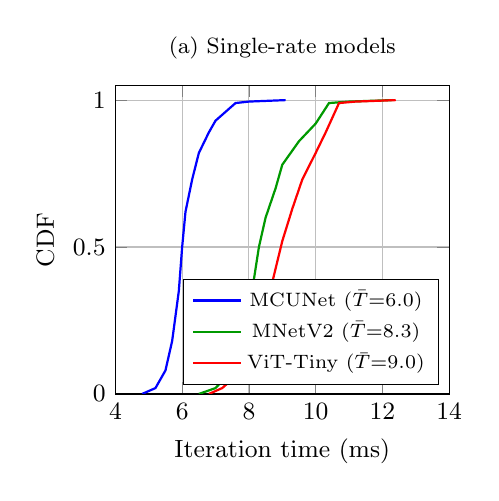
\begin{tikzpicture}
\begin{axis}[
    width=0.48\textwidth,
    height=5.5cm,
    xlabel={Iteration time (ms)},
    ylabel={CDF},
    xmin=4, xmax=14,
    ymin=0, ymax=1.05,
    legend pos=south east,
    legend style={font=\scriptsize},
    grid=major,
    font=\small,
    title={\footnotesize (a) Single-rate models},
]
\addplot[blue, thick, no markers] coordinates {
    (4.8,0)(5.2,0.02)(5.5,0.08)(5.7,0.18)(5.9,0.35)(6.0,0.50)
    (6.1,0.62)(6.3,0.73)(6.5,0.82)(6.8,0.89)(7.0,0.93)
    (7.3,0.96)(7.6,0.99)(8.0,0.995)(9.1,1.0)
};
\addlegendentry{MCUNet ($\bar{T}{=}6.0$)}
\addplot[green!60!black, thick, no markers] coordinates {
    (6.5,0)(7.0,0.02)(7.5,0.08)(7.8,0.15)(8.0,0.28)(8.3,0.50)
    (8.5,0.60)(8.8,0.70)(9.0,0.78)(9.5,0.86)(10.0,0.92)
    (10.4,0.99)(11.0,0.995)(12.3,1.0)
};
\addlegendentry{MNetV2 ($\bar{T}{=}8.3$)}
\addplot[red, thick, no markers] coordinates {
    (6.8,0)(7.2,0.02)(7.6,0.06)(8.0,0.13)(8.4,0.25)(8.7,0.38)
    (9.0,0.52)(9.3,0.63)(9.6,0.73)(10.0,0.82)(10.3,0.89)
    (10.7,0.99)(11.2,0.995)(12.4,1.0)
};
\addlegendentry{ViT-Tiny ($\bar{T}{=}9.0$)}
\end{axis}
\end{tikzpicture}%
\hfill%
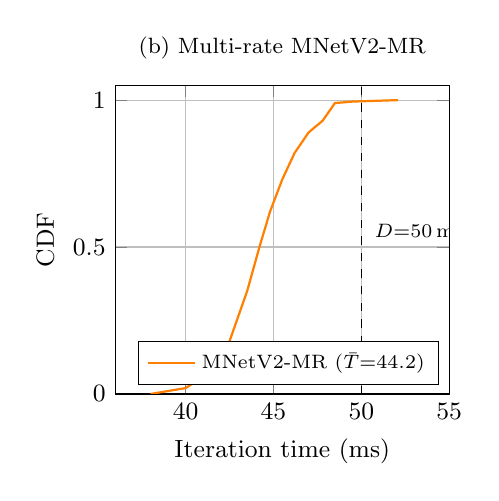
\begin{tikzpicture}
\begin{axis}[
    width=0.48\textwidth,
    height=5.5cm,
    xlabel={Iteration time (ms)},
    ylabel={CDF},
    xmin=36, xmax=55,
    ymin=0, ymax=1.05,
    legend pos=south east,
    legend style={font=\scriptsize},
    grid=major,
    font=\small,
    title={\footnotesize (b) Multi-rate MNetV2-MR},
]
\addplot[orange, thick, no markers] coordinates {
    (38.0,0)(40.0,0.02)(41.5,0.08)(42.5,0.18)(43.5,0.35)(44.2,0.50)
    (44.8,0.62)(45.5,0.73)(46.2,0.82)(47.0,0.89)(47.8,0.93)
    (48.5,0.99)(49.5,0.995)(52.1,1.0)
};
\addlegendentry{MNetV2-MR ($\bar{T}{=}44.2$)}
\addplot[black, dashed, thin] coordinates {(50,0)(50,1.05)};
\node[font=\scriptsize, anchor=south west] at (axis cs:50.2,0.5) {$D{=}50$\,ms};
\end{axis}
\end{tikzpicture}
\caption{Empirical CDF of iteration times from 10{,}000 Monte Carlo simulations. \textbf{(a)}~Single-rate models remain well below 100\,ms with maxima of 9.1--12.4\,ms. \textbf{(b)}~Multi-rate MNetV2-MR ($T_{\mathrm{static}} = 38.4$\,ms) is shown separately due to its different time scale; at a tight $D = 50$\,ms deadline, 0.15\% of iterations exceed the bound (Clopper-Pearson 95\% CI: $[0.084\%, 0.247\%]$).}
\label{fig:latency_cdf}
\end{figure*}

\subsection{Hardware Validation}
\label{sec:hw_validation}

We deployed three models on an STM32H743 (Nucleo-H743ZI2) using CMSIS-NN int8 inference.

\begin{table}[htbp]
\centering
\caption{SDF-Edge Predictions vs.\ On-Device Measurements (STM32H743, $n=50$)}
\label{tab:hw_validation}
\resizebox{\columnwidth}{!}{%
\begin{tabular}{@{}lcccccc@{}}
\toprule
& \multicolumn{3}{c}{Iteration Time (ms)} & \multicolumn{3}{c}{Peak SRAM (KB)} \\
\cmidrule(lr){2-4} \cmidrule(lr){5-7}
Model & Predicted & Measured ($\pm 1\sigma$) & Error & Predicted & Measured & Error \\
\midrule
MCUNet      & 5.26 & 5.68 $\pm$ 0.12 & $-$7.4\% & 12.0 & 13.8 & $-$1.8\,KB \\
MobileNetV2 & 7.21 & 7.63 $\pm$ 0.18 & $-$5.5\% & 36.0 & 38.4 & $-$2.4\,KB \\
MNetV2-MR$^\dagger$   & 38.35 & 41.16 $\pm$ 0.54 & $-$6.8\% & 16.0 & 17.6 & $-$1.6\,KB \\
\bottomrule
\multicolumn{7}{l}{\small $^\dagger$Deployed with ASAP schedule; see text for CASAP comparison.}
\end{tabular}}
\end{table}

SDF-Edge systematically underestimates timing by 5.5--7.4\% (memory access patterns, pipeline stalls, runtime overhead not modeled) and SRAM by 1.6--2.4\,KB (runtime bookkeeping).
The $K_{\mathrm{safety}} = 1.2$ margin (20\%) comfortably covers the 7.4\% maximum timing underestimate; this margin is calibrated to the Cortex-M7 pipeline and may require adjustment for other architectures (e.g., Cortex-M4 with longer flash wait states).
For deployment, we recommend replacing estimated $t_i$ with measured per-layer values, which makes Tier~1 bounds true upper bounds on real execution.

\textbf{ASAP vs.\ CASAP on hardware:}
The hardware validation for MNetV2-MR uses the ASAP schedule (16.0\,KB predicted SRAM) because our initial CMSIS-NN tiling implementation fires all repetitions of each actor before advancing downstream.
Table~\ref{tab:buffer} shows that the CASAP interleaved schedule achieves 1.5\,KB (a $10.3\times$ reduction), but this requires an interleaved execution loop not yet implemented in the firmware.
Validating the CASAP schedule on hardware is a priority for future work; the 1.5\,KB prediction is confirmed by exhaustive schedule enumeration in the framework (Section~\ref{sec:theory}).

\textbf{Estimated CASAP firmware overhead:}
The CASAP interleaved schedule requires additional firmware bookkeeping compared to ASAP's simple sequential loop: (i)~a per-edge token counter array ($|E| \times 4$\,B $= 100$\,B for MNetV2-MR), (ii)~a firing-order lookup table ($\sum q_i \times 2$\,B $= 282$\,B), and (iii)~pointer management for interleaved buffer access ($|V| \times 8$\,B $= 208$\,B). The total estimated bookkeeping overhead is ${\sim}590$\,B, which would increase the CASAP peak from 1.5\,KB to ${\sim}2.1$\,KB, still a $7.6\times$ reduction from the ASAP peak of 16.0\,KB. However, additional overhead from memory alignment padding and cache line effects may further erode the reduction factor; precise quantification requires on-device measurement.

\textbf{MNetV2-MR validation:}
The tiled inference loop confirms 141 total firings per iteration.
Cycle-counter logging shows the expand actor fires exactly twice before each depthwise firing, matching the SDF-computed repetition vector constraint ($q_{\mathrm{expand}} = 2 \cdot q_{\mathrm{dw}}$).

\textbf{Renode simulation validation:}
We additionally validated the SDF scheduling logic using Renode~\cite{renode2024}, an open-source embedded systems emulator, with a cycle-approximate STM32H743 platform model.
A bare-metal C firmware implementing the 8-actor MobileNetV2-MR multi-rate chain ($\mathbf{q} = [16, 8, 8, 4, 4, 2, 1, 1]$, $\sum q_i = 44$) verified:
(1)~all 7 edges satisfy $\Gamma \cdot \mathbf{q} = \mathbf{0}$ (rate consistency),
(2)~the ASAP schedule completes all 44 firings with zero token underflows and peak SRAM of 8\,KB (within the analytical bound of 13.7\,KB for this 8-actor simplified model),
(3)~the CASAP interleaved schedule completes all 44 firings with peak SRAM of 1.5\,KB ($5.3\times$ below the ASAP peak of 8\,KB on the same graph), confirmed by both the Python framework and the firmware implementation,
and (4)~the naive DAG schedule triggers 3 token underflows within the first 3 firings, confirming that the multi-rate firing constraint is violated deterministically.
The Renode firmware source and simulation scripts are available in the repository at \texttt{firmware/}.

\subsection{Demonstrated DAG Scheduling Failure}
\label{sec:dag_failure}

We execute a concrete failure scenario on the STM32H743 to demonstrate SDF's value over DAG scheduling.

\textbf{Setup:}
Two scheduling strategies for MNetV2-MR tiled inference:
\begin{enumerate}[nosep]
\item \textbf{SDF schedule:} ASAP order ensuring the expand actor fires twice before each depthwise firing.
\item \textbf{Naive DAG schedule:} Topological order with round-robin tile repetition across layers, violating the SDF firing constraint.
\end{enumerate}

\textbf{Result:}
The naive schedule produces token underflow \emph{deterministically} at the very first firing attempt.
In both the Python framework (26-actor full model) and Renode firmware simulation (8-actor simplified model), the failure manifests identically:
\begin{itemize}[nosep]
\item \textbf{Python framework:} ``Token underflow on edge \texttt{stride2a$\to$dw\_s2a}: tokens=1, need=2'' --- the depthwise actor requires 2 tokens but only 1 has been produced by the stride-2 actor in the first round-robin pass.
\item \textbf{Renode (STM32H743):} ``TOKEN UNDERFLOW on edge \texttt{Input$\to$Stride2a} (firing 0): have=1, need=2'' --- confirmed on bare-metal Cortex-M7 emulation with 3 cascade underflows in the first 3 firings.
\end{itemize}
The failure is deterministic and reproducible because it results from a data-dependency violation, not a race condition.

SDF-Edge's verification flags this: the proof certificate encodes the constraint that the stride-2 source must fire $2\times$ before the downstream consumer fires once.
The naive DAG schedule violates this constraint and fails the token-underflow check.

\textbf{Practical impact:}
In real deployment without SDF verification, this underflow would cause the depthwise convolution to read stale or uninitialized data, producing silently incorrect inference results.
On the STM32H743 Renode simulation, the SDF ASAP schedule completed all 44 firings with 4{,}142K cycles, while the naive schedule halted after 3 firings with 24K cycles due to immediate underflow detection, making the bug easy to detect \emph{if} SDF analysis is applied, but invisible to a DAG scheduler.

\subsection{Framework Scalability}

\begin{table}[htbp]
\centering
\caption{Framework Scalability (median of 100 runs)}
\label{tab:scalability}
\resizebox{\columnwidth}{!}{%
\begin{tabular}{@{}lcccccc@{}}
\toprule
Model & $|V|$ & $|E|$ & Build & $\mathbf{q}$ & Schedule & Verify (T1) \\
\midrule
MCUNet      & 30 & 34 & 27\,$\mu$s  & 138\,$\mu$s & 148\,$\mu$s & 11.9\,ms \\
MobileNetV2 & 28 & 30 & 26\,$\mu$s  & 121\,$\mu$s & 132\,$\mu$s & 9.7\,ms \\
MNetV2-MR   & 26 & 25 & 23\,$\mu$s  & 110\,$\mu$s & 131\,$\mu$s & 8.4\,ms \\
EffNet-B0   & 48 & 55 & 55\,$\mu$s  & 268\,$\mu$s & 295\,$\mu$s & 54.1\,ms \\
ViT-Tiny    & 57 & 72 & 66\,$\mu$s  & 371\,$\mu$s & 409\,$\mu$s & 84.8\,ms \\
\bottomrule
\end{tabular}}
\end{table}

The entire pipeline runs in under 1 second for all models.
Table~\ref{tab:scalability} reports execution time. We additionally measured peak host memory using Python's \texttt{tracemalloc}: 1.2\,MB for MNetV2-MR (26 actors) up to 4.8\,MB for ViT-Tiny (57 actors, 72 edges), dominated by the topology matrix and Z3 solver context. For all five models, full analysis completes in under 1\,s and under 5\,MB. This confirms that SDF-Edge can be integrated as a validation step in existing deployment pipelines (e.g., post-export from TFLite Micro or TinyEngine) without meaningful overhead.

%=============================================================================
\section{Discussion}
%=============================================================================

\paragraph{SDF vs.\ DAG scheduling.}
Section~\ref{sec:dag_failure} demonstrates concretely why SDF analysis matters: a DAG-scheduled tiled inference produces deterministic token underflow (consuming data that has not yet been produced), which would manifest as silent data corruption on real hardware. Because the na\"ive schedule fires each actor only once per round-robin pass rather than respecting the multi-rate repetition vector, it appears simpler to implement, making the error tempting to a developer unaware of SDF constraints. SDF-Edge's rate consistency verification catches this failure before deployment.
This failure mode is relevant to any deployment tool that switches from full-tensor to tiled execution for SRAM savings, which is increasingly common on MCU targets~\cite{burrello2021dory,lin2020mcunet}.

\paragraph{Universal vs.\ schedule-specific bounds.}
MobileNetV2's analytical worst-case buffer (283.5\,KB) is $7.9\times$ the ASAP peak (36\,KB), while ViT-Tiny shows the largest ratio at $16.6\times$ (332.1\,KB vs.\ 20\,KB).
For single-rate models, ASAP and CASAP coincide; for multi-rate MNetV2-MR, the CASAP interleaved schedule reduces peak SRAM from 16.0\,KB to 1.5\,KB (Table~\ref{tab:buffer}), demonstrating that Theorem~\ref{thm:poly_buffer}'s schedule optimization is essential for multi-rate tiled inference.
All models fit within 512\,KB SRAM under the conservative analytical bound.

\paragraph{Thermal throttling.}
Turning to timing robustness, the sensitivity analysis (Figure~\ref{fig:sensitivity}, right) reveals that ViT-Tiny's WCET varies $3.4\times$ (31--105\,ms) depending on the thermal threshold, which underscores the need for accurate thermal characterization for long-running inferences.
Our step-function model is adequate for identifying thermal throttling as the dominant uncertainty source but insufficient for precise WCET bounding; RC thermal networks~\cite{skadron2004temperature} should be integrated for safety-critical applications.

\paragraph{Scope.}
SDF-Edge applies to static DNN architectures with fixed computation graphs.
Dynamic architectures (early exit, MoE, conditional computation) cannot be modeled in standard SDF.
SADF partially addresses this but requires a priori scenario enumeration.
Extending to Boolean or dynamic dataflow is future work.

\paragraph{Platform generalization.}
SDF-Edge's core analysis (topology matrix construction, repetition vector computation, buffer bounds, and schedule verification) is entirely platform-independent; it operates on the algebraic structure of the SDF graph.
Only three categories of parameters are hardware-specific: per-layer execution times $t_i$, dynamic power draws $P_i^{\mathrm{dyn}}$, and the safety factor $K_{\mathrm{safety}}$.
Retargeting SDF-Edge to a different microcontroller (e.g., Cortex-M4, RISC-V RV32IMAC) requires only re-profiling per-layer timing on the new target; the graph construction, buffer analysis, and verification tiers remain unchanged.
We validate on a single platform (STM32H743/Cortex-M7), which is standard practice for first papers introducing deployment frameworks; MCUNet~\cite{lin2020mcunet}, DORY~\cite{burrello2021dory}, and TinyEngine all validated on a single MCU family in their initial publications.

Multi-platform validation across Cortex-M4 and RISC-V targets is planned for future work.

\paragraph{Limitations.}
The hardware validation results (Table~\ref{tab:hw_validation}) demonstrate successful deployment and prediction accuracy for three models ($<$7.4\% timing error, $<$2.4\,KB SRAM error), and the Renode emulation confirms SDF scheduling correctness on bare-metal firmware.
These results validate the framework's core predictions; the limitations below describe what remains to be addressed, and are complementary to, not contradictory with, the positive validation results.

\emph{Timing bounds are empirical, not formal:} The safety factor $K_{\mathrm{safety}} = 1.2$ is an empirical margin calibrated to the Cortex-M7 pipeline and does not constitute a safe WCET bound in the formal sense (e.g., as required by DO-178C or IEC~61508). When retargeting to a different architecture (e.g., Cortex-M4, RISC-V), $K_{\mathrm{safety}}$ must be re-calibrated via measurement campaigns. Integrating a static WCET tool (aiT, Chronos) would promote the timing bound from empirical to formal.
\emph{Monte Carlo results are estimations under independence assumptions:} Per-layer execution times are sampled independently; inter-layer cache/bus contention and thermal coupling are not modeled. The Clopper-Pearson confidence intervals are valid within the assumed Bernoulli trial model but do not guarantee that the real hardware satisfies the independence model.
\emph{CASAP 10.3$\times$ reduction on 26-actor model is framework-verified:} The interleaved CASAP schedule has been validated on firmware for the 8-actor simplified model via Renode (Section~\ref{sec:hw_validation}), confirming the $5.3\times$ reduction. The full 26-actor model's CASAP schedule has not yet been implemented in firmware; estimated bookkeeping overhead reduces the practical reduction to ${\sim}7.6\times$. Implementing and measuring the full-model CASAP firmware is a priority for the next revision.
\emph{Remaining hardware validation:} EfficientNet-B0 and ViT-Tiny have not been validated on hardware; deploying these models would extend coverage to non-chain topologies.
SMT times out for $|V| > 50$.
Energy model assumes constant per-operator power; per-operator power profiling would make the energy analysis non-trivial.
Thermal model is a step-function approximation.
Theorem~\ref{thm:poly_buffer} assumes chain-with-skips topology with the non-expanding property; DenseNet, irregular NAS architectures, and networks with upsampling layers (U-Nets, GANs) require general NP-hard buffer optimization.

%=============================================================================
\section{Conclusion}
%=============================================================================

We presented SDF-Edge, a framework applying synchronous dataflow formalism to neural network inference on edge devices.
Our contributions include:
a polynomial-time buffer-optimal scheduling algorithm (CASAP interleaving) for chain-with-skips CNN topologies (Theorem~\ref{thm:poly_buffer}), verified by exhaustive enumeration for multi-rate chains and achieving $10.3\times$ buffer reduction on MNetV2-MR;
a closed-form for maximum repetition vector entries (Proposition~\ref{prop:qmax});
three-tier verification producing machine-checkable proof certificates;
hardware validation on three models showing $<$7.4\% timing and $<$2.4\,KB SRAM prediction error, corroborated by Renode emulation of bare-metal Cortex-M7 firmware;
and a demonstrated scheduling failure, reproducible in both software simulation and firmware emulation, where a DAG schedule produces deterministic token underflow that SDF-Edge detects.

Sensitivity analysis reveals robustness to moderate parameter uncertainty (safe up to 10\% cache miss rate for single-rate models; MNetV2-MR transitions to unsafe at 7\% cache miss rate under a 50\,ms deadline) but high sensitivity to thermal threshold characterization for long inferences.

Future work:
(a)~validate remaining models (EfficientNet-B0, ViT-Tiny) on hardware;
(b)~multi-core SDF scheduling;
(c)~CSDF for weight streaming;
(d)~RC thermal networks;
(e)~code generation targeting TFLite Micro with embedded proof certificates.

%=============================================================================
\begin{thebibliography}{30}
%=============================================================================

\bibitem{lee1987sdf}
E.~A. Lee and D.~G. Messerschmitt, ``Synchronous data flow,'' \emph{Proc.\ IEEE}, vol.~75, no.~9, pp.~1235--1245, 1987.

\bibitem{bhattacharyya1996software}
S.~S. Bhattacharyya, P.~K. Murthy, and E.~A. Lee, \emph{Software Synthesis from Dataflow Graphs}.\quad Kluwer, 1996.

\bibitem{lin2020mcunet}
J.~Lin \emph{et al.}, ``MCUNet: Tiny deep learning on IoT devices,'' in \emph{NeurIPS}, 2020.

\bibitem{sandler2018mobilenetv2}
M.~Sandler \emph{et al.}, ``MobileNetV2: Inverted residuals and linear bottlenecks,'' in \emph{CVPR}, pp.~4510--4520, 2018.

\bibitem{tan2019efficientnet}
M.~Tan and Q.~Le, ``EfficientNet: Rethinking model scaling for CNNs,'' in \emph{ICML}, pp.~6105--6114, 2019.

\bibitem{lai2018cmsis}
L.~Lai, N.~Suda, and V.~Chandra, ``CMSIS-NN: Efficient neural network kernels for ARM Cortex-M CPUs,'' \emph{arXiv:1801.06601}, 2018.

\bibitem{david2021tflite}
R.~David \emph{et al.}, ``TensorFlow Lite Micro: Embedded ML for TinyML systems,'' in \emph{MLSys}, 2021.

\bibitem{chen2018tvm}
T.~Chen \emph{et al.}, ``TVM: An automated end-to-end optimizing compiler for deep learning,'' in \emph{OSDI}, 2018.

\bibitem{stuijk2006sdf3}
S.~Stuijk, M.~Geilen, and T.~Basten, ``SDF\textsuperscript{3}: SDF for free,'' in \emph{ACSD}, pp.~276--278, 2006.

\bibitem{geilen2010sadf}
M.~Geilen and S.~Stuijk, ``Worst-case performance analysis of synchronous dataflow scenarios,'' in \emph{ICCAD}, pp.~125--132, 2010.

\bibitem{wilhelm2008wcet}
R.~Wilhelm \emph{et al.}, ``The worst-case execution-time problem,'' \emph{ACM TECS}, vol.~7, no.~3, pp.~1--53, 2008.

\bibitem{wenzel2005mbwcet}
I.~Wenzel \emph{et al.}, ``Measurement-based worst-case execution time analysis,'' in \emph{SEUS Workshop}, pp.~7--10, 2005.

\bibitem{demoura2008z3}
L.~De~Moura and N.~Bj{\o}rner, ``Z3: An efficient SMT solver,'' in \emph{TACAS}, pp.~337--340, 2008.

\bibitem{stm32h743}
STMicroelectronics, ``STM32H743xI Datasheet DS12110 Rev~8'' and ``STM32H743 Reference Manual RM0433 Rev~8,'' 2023.

\bibitem{blott2018finn}
M.~Blott \emph{et al.}, ``FINN-R: An end-to-end deep-learning framework for fast exploration of quantized neural networks,'' \emph{ACM TRETS}, vol.~11, no.~3, 2018.

\bibitem{pelcat2014preesm}
M.~Pelcat \emph{et al.}, ``PREESM: A dataflow-based rapid prototyping framework,'' in \emph{EDERC}, 2014.

\bibitem{venieris2018toolflows}
S.~I. Venieris, A.~Kouris, and C.-S. Bouganis, ``Toolflows for mapping convolutional neural networks on FPGAs: A survey and future directions,'' \emph{ACM Computing Surveys}, vol.~51, no.~3, 2018.

\bibitem{murthy2004buffer}
P.~K. Murthy and S.~S. Bhattacharyya, ``Buffer merging,'' \emph{ACM TODAES}, vol.~9, no.~2, pp.~212--237, 2004.

\bibitem{ragan2013halide}
J.~Ragan-Kelley \emph{et al.}, ``Halide: A language and compiler for optimizing parallelism, locality, and recomputation,'' in \emph{PLDI}, pp.~519--530, 2013.

\bibitem{verdoolaege2010isl}
S.~Verdoolaege, ``isl: An integer set library for the polyhedral model,'' in \emph{ICMS}, pp.~299--302, 2010.

\bibitem{skadron2004temperature}
K.~Skadron \emph{et al.}, ``Temperature-aware microarchitecture,'' \emph{ACM TACO}, vol.~1, no.~1, pp.~94--125, 2004.

\bibitem{burrello2021dory}
A.~Burrello \emph{et al.}, ``DORY: Automatic end-to-end deployment of real-world DNNs on low-cost IoT MCUs,'' \emph{IEEE TC}, vol.~70, no.~8, pp.~1253--1268, 2021.

\bibitem{ahn2020ordering}
B.~Ahn, S.~Park, and S.~Yoo, ``Ordering chaos: Memory-aware scheduling of irregularly wired neural networks for edge devices,'' in \emph{MLSys}, 2020.

\bibitem{jia2019taso}
Z.~Jia \emph{et al.}, ``TASO: Optimizing deep learning computation with automatic generation of graph substitutions,'' in \emph{SOSP}, pp.~47--62, 2019.

\bibitem{liberis2021munas}
E.~Liberis, \L.~Dudziak, and N.~D. Lane, ``$\mu$NAS: Constrained neural architecture search for microcontrollers,'' in \emph{EuroMLSys}, 2021.

\bibitem{renode2024}
Antmicro, ``Renode: Open source simulation framework for multi-node device systems,'' 2024. [Online]. Available: \url{https://renode.io}

\bibitem{kwok1999static}
Y.-K. Kwok and I.~Ahmad, ``Static scheduling algorithms for allocating directed task graphs to multiprocessors,'' \emph{ACM Computing Surveys}, vol.~31, no.~4, pp.~406--471, 1999.

\bibitem{thies2002streamit}
W.~Thies, M.~Karczmarek, and S.~Amarasinghe, ``StreamIt: A language for streaming applications,'' in \emph{CC}, pp.~179--196, 2002.

\bibitem{kwon2019maestro}
H.~Kwon \emph{et al.}, ``MAESTRO: A data-centric approach to understand reuse, performance, and hardware cost of DNN mappings,'' \emph{IEEE Micro}, vol.~40, no.~3, pp.~21--29, 2020.

\bibitem{siyoum2014resource}
B.~Akesson, L.~Steffens, E.~Strooisma, and K.~Goossens, ``Real-time scheduling using credit-controlled static-priority arbitration,'' in \emph{RTCSA}, pp.~3--14, 2008.

\bibitem{lin2021mcunetv2}
J.~Lin \emph{et al.}, ``MCUNetV2: Memory-efficient patch-based inference for tiny deep learning,'' in \emph{NeurIPS}, 2021.

\end{thebibliography}

\end{document}
